\section{Implémentation}
\subsection{Présentation du jeu}
Comme dit précédemment, notre jeu est un jeu de type puzzle en 2D en vue du dessus. Notre jeu compte 25 niveaux de  bases, il est possible de créer nos propres niveau et de les inclure dans notre liste de niveaux. Pour terminer un niveau (et donc finir le puzzle), il faut mettre toutes les caisses sur une platforme, les platformes ne sont pas spécifiques à une caisse.

\subsection{Présentation de l'UI}
\subsubsection{Ecran titre}
	\begin{figure}[h]
	  \centering
	  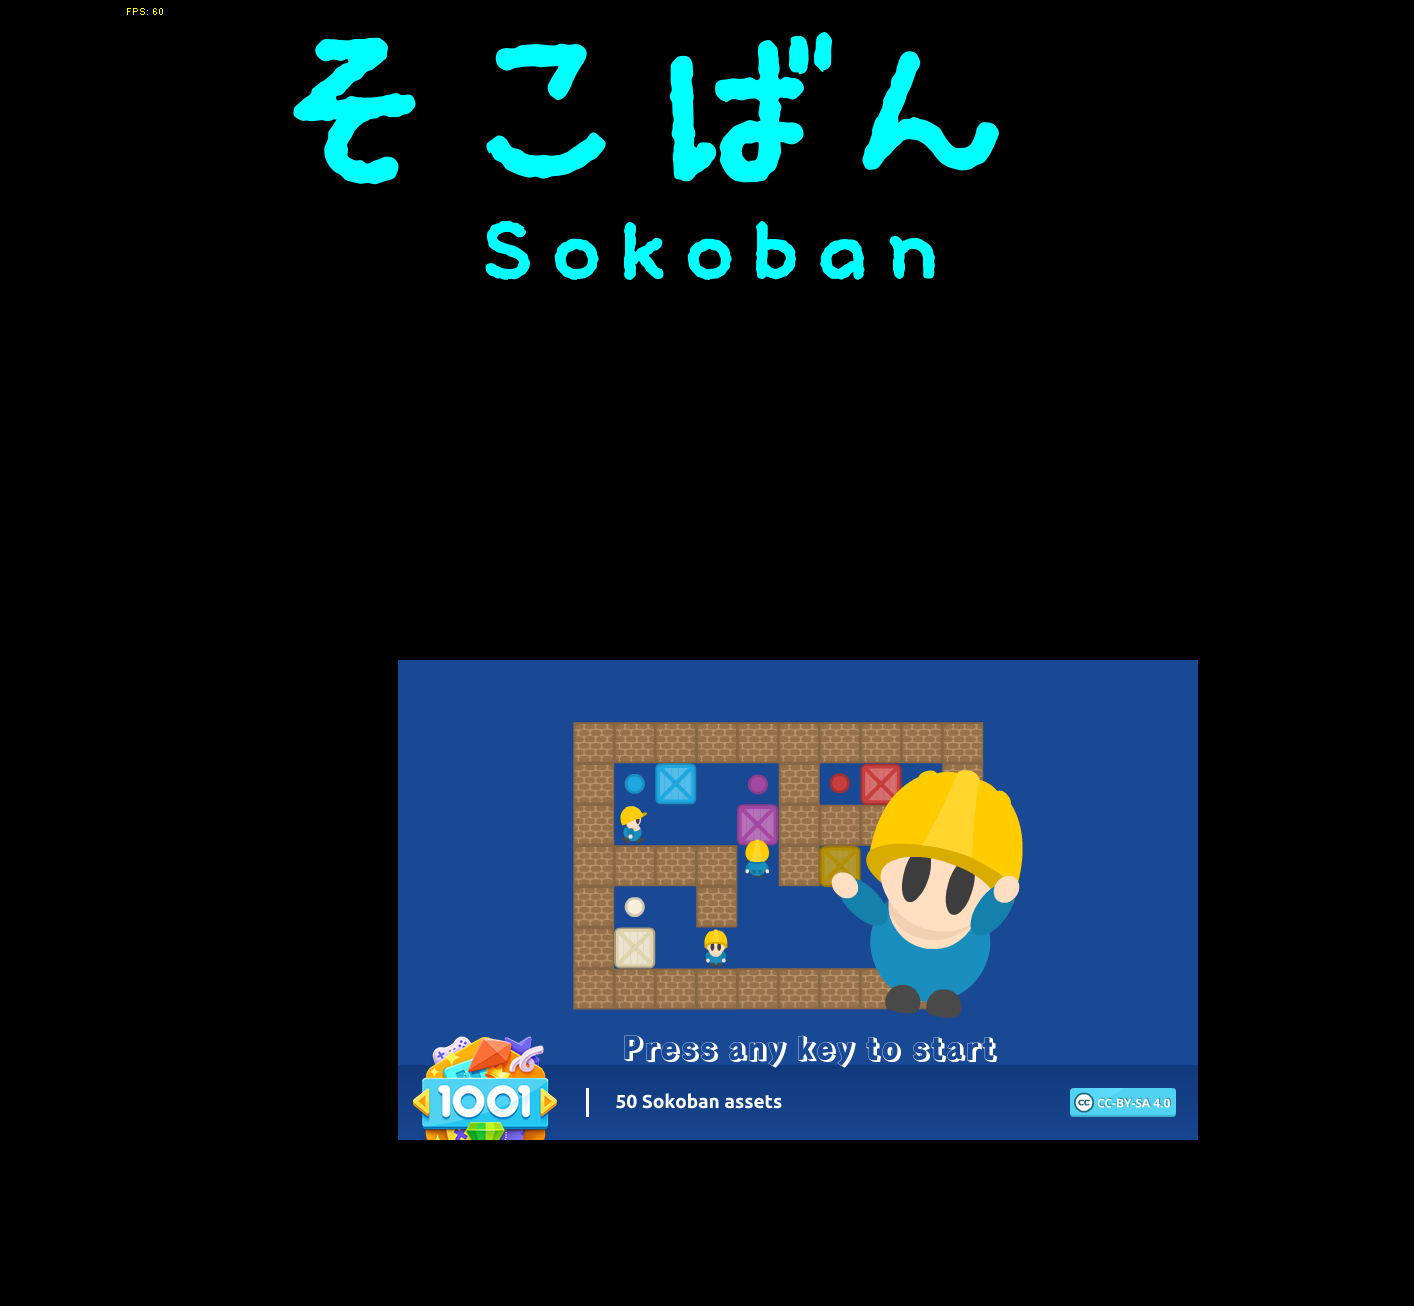
\includegraphics[width=0.5\textwidth] {pictures/title_screen.png}
	  \caption{écran titre}
	  \label{fig:title_screen}
	\end{figure}
Voici à quoi ressemble l'écran titre de notre jeu, comme vous pouvez le remarquer, l'écran titre est composé du nom de l'application (écrit en alphabet latin et en japonais). Une image de présentation du jeu est également présente.

\subsubsection{Menu principal}
	\begin{figure}[h]
	  \centering
	  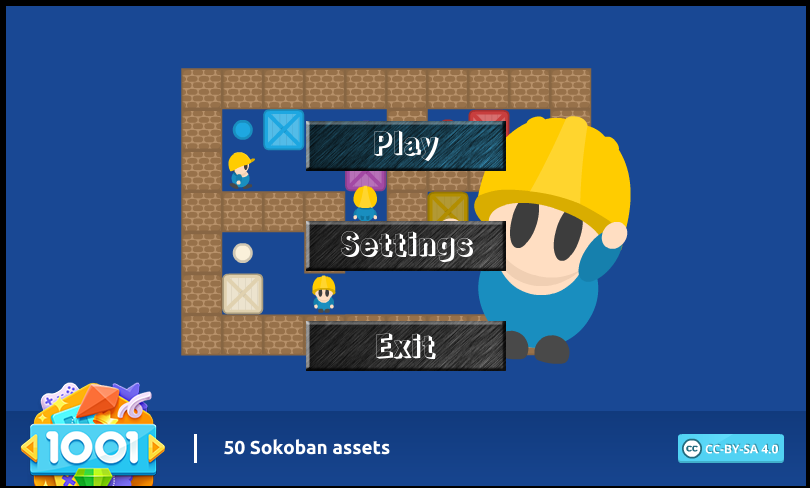
\includegraphics[width=0.5\textwidth] {pictures/main_menu.png}
	  \caption{menu principal}
	  \label{fig:main_menu}
	\end{figure}
Notre menu principal est composé de trois bouttons , Le premier permettant de jouer, le deuxième permet d'accéder au menu "paused" et le troisième permet de quitter le jeu. L'image de 
fond reste la même qu'à l'écran titre.

\newpage
\subsubsection{Menu pause}
	\begin{figure}[h]
	  \centering
	  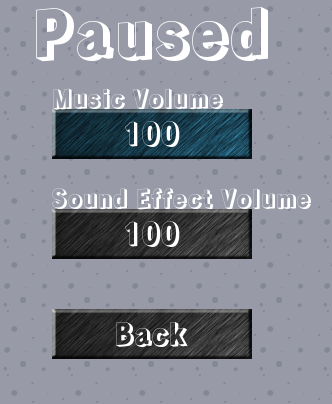
\includegraphics[width=0.3\textwidth] {pictures/paused_menu.png}
	  \caption{menu pause}
	  \label{fig:paused_menu}
	\end{figure}
Les deux premiers bouttons permettent de régler le volume de la musique et le volume des effets sonores. Pour modifier les valeurs, sélectionné le bouton correspondant grâce au flèche haut et bas du 
clavier. Appuyez sur la touche "enter" et appuyez sur la flèche du haut pour monter le volume ou celle du bas pour le descendre. Une fois le modification faite appuyez sur "esc" pour sortir de la
sélection du boutton. Le dernier boutton permet de reprendre le jeu où il a été laissé.

\subsubsection{Jeu}
	\begin{figure}[h]
	  \centering
	  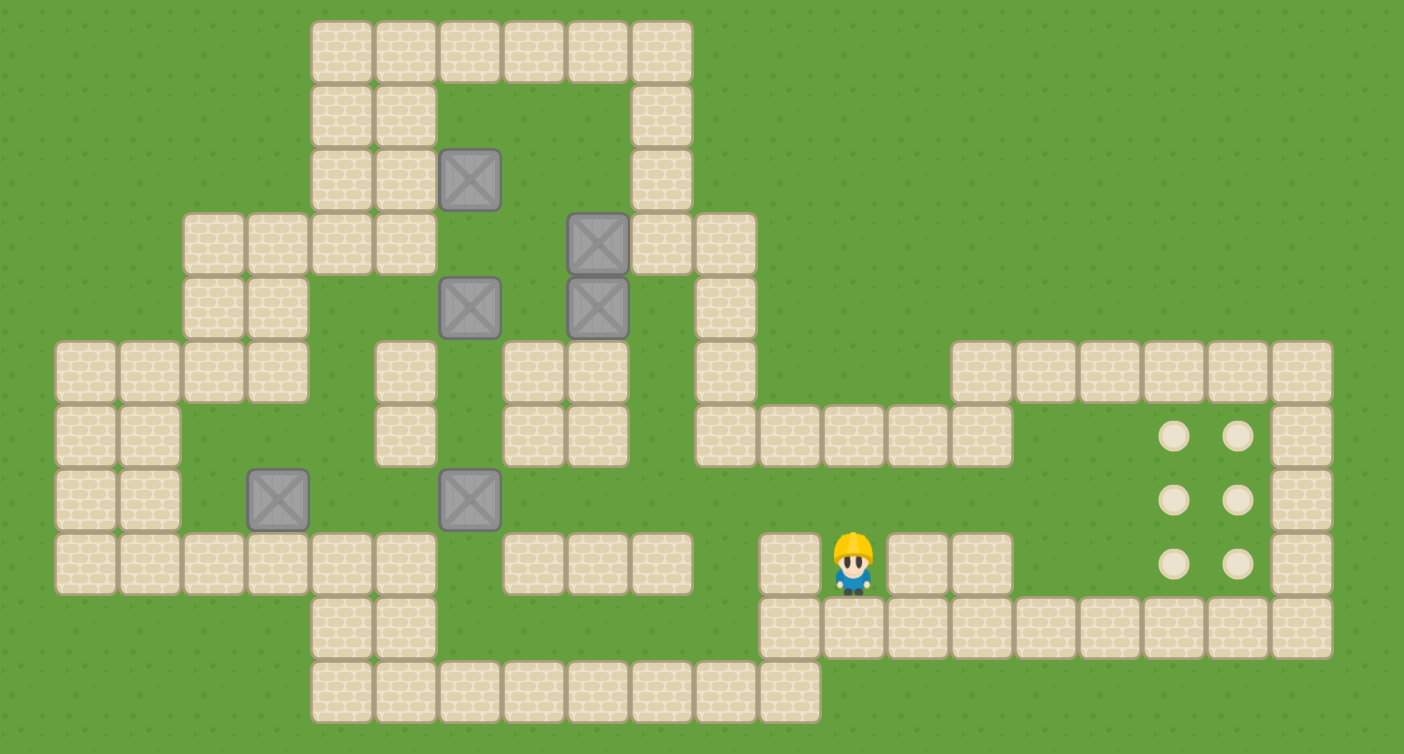
\includegraphics[width=0.7\textwidth] {pictures/jeu.png}
	  \caption{jeu}
	  \label{fig:jeu}
	\end{figure}
Voici à quoi ressemble notre jeu. La vue est composé d'un fond à pois (vert sur l'image), de murs qui définissent la limite de la zone du puzzle (beiges sur l'image), de platformes qui définissent 
l'emplacement de l'objectif (blanches sur l'image) et de caisses (grises sur l'image )qui doivent être déplacées vers les objectifs (blancs sur l'image). les couleurs changent de manière aléatoire pour chaque reset de niveau.
